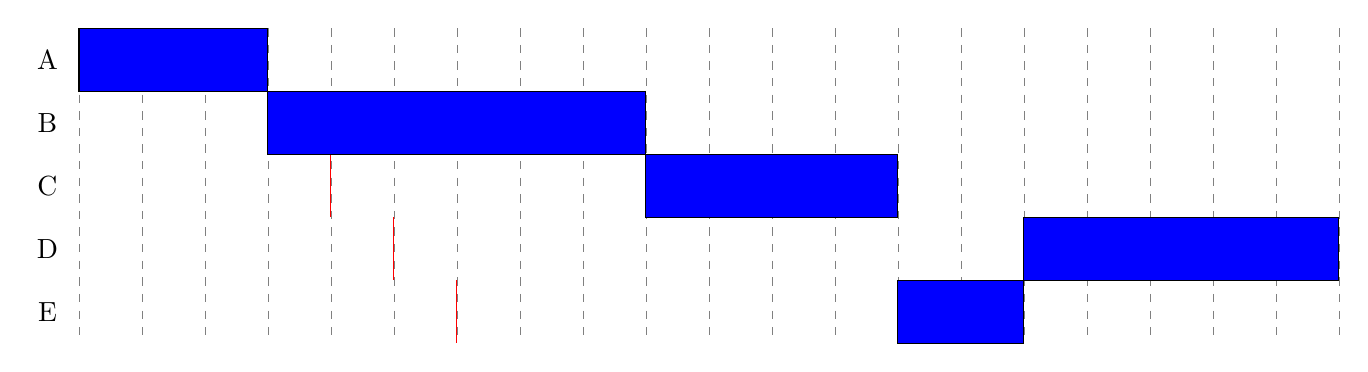
\begin{tikzpicture}[scale=.8]
   \foreach \i in {0,...,20}
   \draw[dashed, help lines] (\i,0) -- (\i,-5);

   \node (A) at (-.5,-.5) {A};
   \node (B) at (-.5,-1.5) {B};
   \node (C) at (-.5,-2.5) {C};
   \node (D) at (-.5,-3.5) {D};
   \node (E) at (-.5,-4.5) {E};

   \foreach \p in {0,...,4}
   \draw[red] (2+\p, -\p) --++ (0,-1);

   \draw[fill=blue] (0,0) rectangle (3,-1) rectangle (9,-2);
   \draw[fill=blue] (9,-2) rectangle (13,-3);
   \draw[fill=blue] (13,-5) rectangle (15,-4) rectangle (20,-3);

\end{tikzpicture}

%Tt      3  9     13    20    19    //
%Tr      3  7     9     14    7     8
%Tr/Ts   1  3/6   9/4   14/5  7/2   2.34